\documentclass[tikz,border=10pt]{standalone}
\usepackage{tikz}
\usetikzlibrary{calc}

\begin{document}

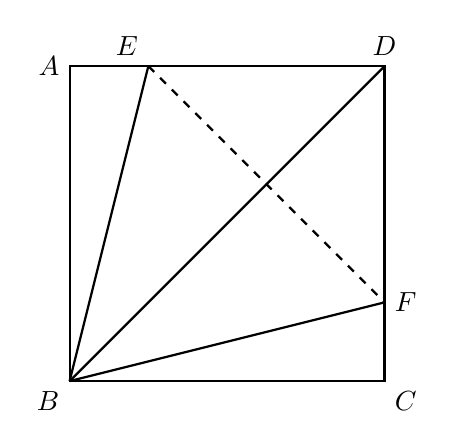
\begin{tikzpicture}[scale=4, thick, >=stealth]
    % 1. 定义正方形的四个顶点
    \coordinate (B) at (0,0);
    \coordinate (C) at (1,0);
    \coordinate (D) at (1,1);
    \coordinate (A) at (0,1);

    % 2. 定义边上的特殊点 E 和 F
    % 根据原图比例：E 在 AD 上约 1/4 处，F 在 CD 上约 1/4 处
    \coordinate (E) at (0.25, 1);
    \coordinate (F) at (1, 0.25);

    % 3. 绘制正方形边界
    \draw (A) -- (B) -- (C) -- (D) -- cycle;

    % 4. 绘制从 B 点出发的实线射线
    \draw (B) -- (E);  % 连接 BE
    \draw (B) -- (D);  % 连接 BD (对角线)
    \draw (B) -- (F);  % 连接 BF

    % 5. 绘制虚线辅助线 EF
    \draw[dashed] (E) -- (F);

    % 6. 标注顶点标签
    % anchor 用于微调文字位置，确保不与线段重叠
    \node[left] at (A) {$A$};
    \node[below left] at (B) {$B$};
    \node[below right] at (C) {$C$};
    \node[above] at (D) {$D$};
    \node[above left] at (E) {$E$};
    \node[right] at (F) {$F$};


\end{tikzpicture}

\end{document}